\documentclass[a4paper,11pt]{article}
\usepackage[utf8]{inputenc}\usepackage[T1]{fontenc}
\usepackage[english]{babel}\usepackage{lmodern}\usepackage{microtype}
\usepackage{amsmath,amssymb}\usepackage{geometry}
\geometry{a4paper,left=2.2cm,right=2.2cm,top=2.0cm,bottom=2.0cm}
\usepackage{booktabs,array}\usepackage{xcolor}
\definecolor{bokug}{RGB}{0,135,60}\usepackage{tikz}
\usetikzlibrary{arrows.meta,calc}
\usepackage{fancyhdr}\pagestyle{fancy}
\renewcommand{\headrulewidth}{0.4pt}
\usepackage{enumitem}\setlength{\parindent}{0pt}\setlength{\parskip}{4pt}

\begin{document}
\fancyhead[L]{\small VU Mechanik – LAWI 100515 (PI)}\fancyhead[R]{\small SS 2026}\fancyfoot[C]{\thepage}
\begin{center}{\large\bfseries\color{bokug}University of Natural Resources and Life Sciences, Vienna (BOKU)}\\[2pt]{\large\bfseries VU Mechanik – LAWI 100515 (PI)}\\[4pt]Exam \textbf{Group A} \hfill Date: 26.06.2026\\[2pt]\rule{\linewidth}{0.4pt}\end{center}

\begin{center}\textbf{\large Model solution}\end{center}
\begin{center}
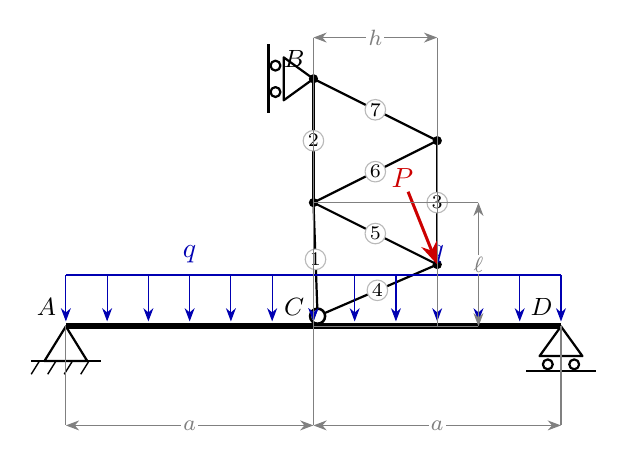
\begin{tikzpicture}[scale=1.048,>=Stealth,line join=round]
  \coordinate (P0) at (0.000,0.000);
  \coordinate (P1) at (3.000,0.000);
  \coordinate (P2) at (6.000,0.000);
  \coordinate (TO1) at (3.000,1.500);
  \coordinate (TO2) at (3.000,3.000);
  \coordinate (TU0) at (4.500,0.750);
  \coordinate (TU1) at (4.500,2.250);
  \coordinate (CPIN) at (3.050,0.124);
  \draw[thick] (CPIN) -- (TO1);
  \draw[thick] (TO1) -- (TO2);
  \draw[thick] (TU0) -- (TU1);
  \draw[thick] (CPIN) -- (TU0);
  \draw[thick] (TU0) -- (TO1);
  \draw[thick] (TO1) -- (TU1);
  \draw[thick] (TU1) -- (TO2);
  \draw[line width=2.2pt] (P0) -- (P1);
  \draw[line width=2.2pt] (P1) -- (P2);
  \fill (TO1) circle (1.6pt);
  \fill (TO2) circle (1.6pt);
  \fill (TU0) circle (1.6pt);
  \fill (TU1) circle (1.6pt);
  \draw[fill=white,line width=0.9pt] (CPIN) circle (2.6pt);
  \draw[thick] (0.000,0.000) -- (-0.260,-0.420) -- (0.260,-0.420) -- cycle;
  \draw[line width=1pt] (-0.420,-0.420) -- (0.420,-0.420);
  \draw[line width=0.5pt] (-0.320,-0.420) -- (-0.420,-0.580);
  \draw[line width=0.5pt] (-0.120,-0.420) -- (-0.220,-0.580);
  \draw[line width=0.5pt] (0.080,-0.420) -- (-0.020,-0.580);
  \draw[line width=0.5pt] (0.280,-0.420) -- (0.180,-0.580);
  \draw[thick] (6.000,0.000) -- (5.740,-0.360) -- (6.260,-0.360) -- cycle;
  \draw[thick] (5.840,-0.460) circle (0.06) (6.160,-0.460) circle (0.06);
  \draw[line width=1pt] (5.580,-0.540) -- (6.420,-0.540);
  \draw[thick] (3.000,3.000) -- (2.640,3.260) -- (2.640,2.740) -- cycle;
  \draw[thick] (2.540,3.160) circle (0.06) (2.540,2.840) circle (0.06);
  \draw[line width=1pt] (2.460,3.420) -- (2.460,2.580);
  \node[circle,fill=white,draw=gray!55,inner sep=0.5pt,font=\scriptsize] at (3.025,0.812) {1};
  \node[circle,fill=white,draw=gray!55,inner sep=0.5pt,font=\scriptsize] at (3.000,2.250) {2};
  \node[circle,fill=white,draw=gray!55,inner sep=0.5pt,font=\scriptsize] at (4.500,1.500) {3};
  \node[circle,fill=white,draw=gray!55,inner sep=0.5pt,font=\scriptsize] at (3.775,0.437) {4};
  \node[circle,fill=white,draw=gray!55,inner sep=0.5pt,font=\scriptsize] at (3.750,1.125) {5};
  \node[circle,fill=white,draw=gray!55,inner sep=0.5pt,font=\scriptsize] at (3.750,1.875) {6};
  \node[circle,fill=white,draw=gray!55,inner sep=0.5pt,font=\scriptsize] at (3.750,2.625) {7};
  \draw[->,blue!70!black] (0.000,0.620) -- (0.000,0.060);
  \draw[->,blue!70!black] (0.500,0.620) -- (0.500,0.060);
  \draw[->,blue!70!black] (1.000,0.620) -- (1.000,0.060);
  \draw[->,blue!70!black] (1.500,0.620) -- (1.500,0.060);
  \draw[->,blue!70!black] (2.000,0.620) -- (2.000,0.060);
  \draw[->,blue!70!black] (2.500,0.620) -- (2.500,0.060);
  \draw[->,blue!70!black] (3.000,0.620) -- (3.000,0.060);
  \draw[blue!70!black,thick] (0.000,0.620) -- (3.000,0.620);
  \node[blue!70!black] at (1.500,0.870) {$q$};
  \draw[->,blue!70!black] (3.000,0.620) -- (3.000,0.060);
  \draw[->,blue!70!black] (3.500,0.620) -- (3.500,0.060);
  \draw[->,blue!70!black] (4.000,0.620) -- (4.000,0.060);
  \draw[->,blue!70!black] (4.500,0.620) -- (4.500,0.060);
  \draw[->,blue!70!black] (5.000,0.620) -- (5.000,0.060);
  \draw[->,blue!70!black] (5.500,0.620) -- (5.500,0.060);
  \draw[->,blue!70!black] (6.000,0.620) -- (6.000,0.060);
  \draw[blue!70!black,thick] (3.000,0.620) -- (6.000,0.620);
  \node[blue!70!black] at (4.500,0.870) {$q$};
  \draw[->,red!80!black,line width=1.1pt] (4.147,1.632) -- (4.500,0.750);
  \node[red!80!black] at (4.080,1.799) {$P$};
  \draw[thin,gray] (0.000,0.000) -- (0.000,-1.200);
  \draw[thin,gray] (3.000,0.000) -- (3.000,-1.200);
  \draw[<->,gray] (0.000,-1.200) -- (3.000,-1.200) node[midway,fill=white,inner sep=0.8pt,font=\footnotesize]{$a$};
  \draw[thin,gray] (3.000,0.000) -- (3.000,-1.200);
  \draw[thin,gray] (6.000,0.000) -- (6.000,-1.200);
  \draw[<->,gray] (3.000,-1.200) -- (6.000,-1.200) node[midway,fill=white,inner sep=0.8pt,font=\footnotesize]{$a$};
  \draw[thin,gray] (3.000,0.000) -- (5.000,0.000);
  \draw[thin,gray] (3.000,1.500) -- (5.000,1.500);
  \draw[<->,gray] (5.000,0.000) -- (5.000,1.500) node[midway,fill=white,inner sep=0.8pt,font=\footnotesize]{$\ell$};
  \draw[thin,gray] (3.000,0.000) -- (3.000,3.500);
  \draw[thin,gray] (4.500,0.000) -- (4.500,3.500);
  \draw[<->,gray] (3.000,3.500) -- (4.500,3.500) node[midway,fill=white,inner sep=0.8pt,font=\footnotesize]{$h$};
  \node[font=\small] at (0.000,0.000) [xshift=-7pt,yshift=7pt] {$A$};
  \node[font=\small] at (3.000,0.000) [xshift=-7pt,yshift=7pt] {$C$};
  \node[font=\small] at (6.000,0.000) [xshift=-7pt,yshift=7pt] {$D$};
  \node[font=\small] at (3.000,3.000) [xshift=-7pt,yshift=7pt] {$B$};
\end{tikzpicture}
\end{center}
\par\medskip\textbf{1.\ Static determinacy}\par Counting criterion $n=3k-(a+z)$ (bodies $k$, reactions $a$, interaction forces $z$):
\[ n=3k-(a+z)=3\cdot2-(4+2)=0\ \Rightarrow\ \text{statically determinate} \]
\par\medskip\textbf{2.\ Support reactions and hinge forces}\par
$A:\ R_x=4,\ R_y=22$\quad $D:\ R_x=0,\ R_y=22$\quad $B:\ R_x=-12,\ R_y=0$\par $C:\ H_x=-4,\ H_y=-20$
\par\medskip\textbf{3.\ Truss member forces}\par
\begin{center}\renewcommand{\arraystretch}{1.1}\begin{tabular}{c r l}
\toprule
Member & Force $S$ [kN] & Type \\
\midrule
  1 & -18 & compression \\
  2 & -6 & compression \\
  3 & 12 & tension \\
  4 & -4.47 & compression \\
  5 & 13.42 & tension \\
  6 & -13.42 & compression \\
  7 & 13.42 & tension \\
\bottomrule
\end{tabular}\end{center}
\begin{center}
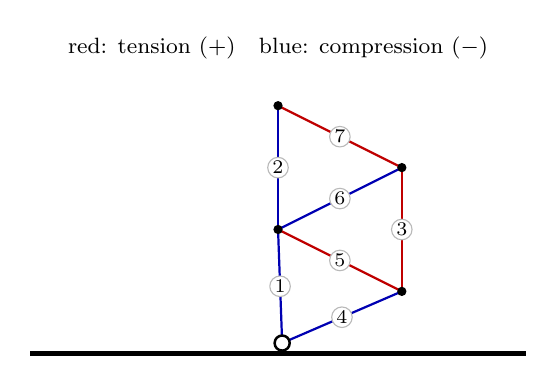
\begin{tikzpicture}[scale=1.048,>=Stealth,line join=round]
  \coordinate (P0) at (0.000,0.000);
  \coordinate (P1) at (3.000,0.000);
  \coordinate (P2) at (6.000,0.000);
  \coordinate (TO1) at (3.000,1.500);
  \coordinate (TO2) at (3.000,3.000);
  \coordinate (TU0) at (4.500,0.750);
  \coordinate (TU1) at (4.500,2.250);
  \coordinate (CPIN) at (3.050,0.124);
  \draw[thick,blue!70!black] (CPIN) -- (TO1);
  \draw[thick,blue!70!black] (TO1) -- (TO2);
  \draw[thick,red!75!black] (TU0) -- (TU1);
  \draw[thick,blue!70!black] (CPIN) -- (TU0);
  \draw[thick,red!75!black] (TU0) -- (TO1);
  \draw[thick,blue!70!black] (TO1) -- (TU1);
  \draw[thick,red!75!black] (TU1) -- (TO2);
  \draw[line width=2pt] (P0) -- (P1);
  \draw[line width=2pt] (P1) -- (P2);
  \fill (TO1) circle (1.6pt);
  \fill (TO2) circle (1.6pt);
  \fill (TU0) circle (1.6pt);
  \fill (TU1) circle (1.6pt);
  \draw[fill=white,line width=0.9pt] (CPIN) circle (2.6pt);
  \node[circle,fill=white,draw=gray!55,inner sep=0.5pt,font=\scriptsize] at (3.025,0.812) {1};
  \node[circle,fill=white,draw=gray!55,inner sep=0.5pt,font=\scriptsize] at (3.000,2.250) {2};
  \node[circle,fill=white,draw=gray!55,inner sep=0.5pt,font=\scriptsize] at (4.500,1.500) {3};
  \node[circle,fill=white,draw=gray!55,inner sep=0.5pt,font=\scriptsize] at (3.775,0.437) {4};
  \node[circle,fill=white,draw=gray!55,inner sep=0.5pt,font=\scriptsize] at (3.750,1.125) {5};
  \node[circle,fill=white,draw=gray!55,inner sep=0.5pt,font=\scriptsize] at (3.750,1.875) {6};
  \node[circle,fill=white,draw=gray!55,inner sep=0.5pt,font=\scriptsize] at (3.750,2.625) {7};
  \node[font=\footnotesize] at (3.00,3.70) {red: tension $(+)$\quad blue: compression $(-)$};
\end{tikzpicture}
\end{center}
\par\medskip\textbf{4.\ Section-force diagrams of the beams}\par
\begin{center}
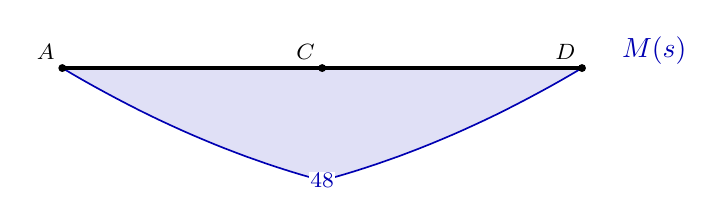
\begin{tikzpicture}[scale=1.100,line join=round]
  \filldraw[fill=blue!70!black!12,draw=blue!70!black,semithick] (0.000,0.000) -- (0.125,-0.074) -- (0.250,-0.146) -- (0.375,-0.216) -- (0.500,-0.284) -- (0.625,-0.351) -- (0.750,-0.416) -- (0.875,-0.480) -- (1.000,-0.542) -- (1.125,-0.602) -- (1.250,-0.660) -- (1.375,-0.717) -- (1.500,-0.772) -- (1.625,-0.825) -- (1.750,-0.877) -- (1.875,-0.927) -- (2.000,-0.975) -- (2.125,-1.022) -- (2.250,-1.066) -- (2.375,-1.110) -- (2.500,-1.151) -- (2.625,-1.191) -- (2.750,-1.229) -- (2.875,-1.265) -- (3.000,-1.300) -- (3.000,-1.300) -- (3.125,-1.265) -- (3.250,-1.229) -- (3.375,-1.191) -- (3.500,-1.151) -- (3.625,-1.110) -- (3.750,-1.066) -- (3.875,-1.022) -- (4.000,-0.975) -- (4.125,-0.927) -- (4.250,-0.877) -- (4.375,-0.825) -- (4.500,-0.772) -- (4.625,-0.717) -- (4.750,-0.660) -- (4.875,-0.602) -- (5.000,-0.542) -- (5.125,-0.480) -- (5.250,-0.416) -- (5.375,-0.351) -- (5.500,-0.284) -- (5.625,-0.216) -- (5.750,-0.146) -- (5.875,-0.074) -- (6.000,0.000) -- (6.000,0.000) -- (5.875,0.000) -- (5.750,0.000) -- (5.625,0.000) -- (5.500,0.000) -- (5.375,0.000) -- (5.250,0.000) -- (5.125,0.000) -- (5.000,0.000) -- (4.875,0.000) -- (4.750,0.000) -- (4.625,0.000) -- (4.500,0.000) -- (4.375,0.000) -- (4.250,0.000) -- (4.125,0.000) -- (4.000,0.000) -- (3.875,0.000) -- (3.750,0.000) -- (3.625,0.000) -- (3.500,0.000) -- (3.375,0.000) -- (3.250,0.000) -- (3.125,0.000) -- (3.000,0.000) -- (3.000,0.000) -- (2.875,0.000) -- (2.750,0.000) -- (2.625,0.000) -- (2.500,0.000) -- (2.375,0.000) -- (2.250,0.000) -- (2.125,0.000) -- (2.000,0.000) -- (1.875,0.000) -- (1.750,0.000) -- (1.625,0.000) -- (1.500,0.000) -- (1.375,0.000) -- (1.250,0.000) -- (1.125,0.000) -- (1.000,0.000) -- (0.875,0.000) -- (0.750,0.000) -- (0.625,0.000) -- (0.500,0.000) -- (0.375,0.000) -- (0.250,0.000) -- (0.125,0.000) -- (0.000,0.000) -- cycle;
  \draw[line width=1.6pt] (0.000,0.000) -- (3.000,0.000) -- (6.000,0.000);
  \node[blue!70!black,font=\footnotesize,fill=white,inner sep=0.5pt] at (3.000,-1.300) {48};
  \fill (0.000,0.000) circle (1.3pt);
  \node[font=\footnotesize] at (0.000,0.000) [xshift=-6pt,yshift=6pt] {$A$};
  \fill (3.000,0.000) circle (1.3pt);
  \node[font=\footnotesize] at (3.000,0.000) [xshift=-6pt,yshift=6pt] {$C$};
  \fill (6.000,0.000) circle (1.3pt);
  \node[font=\footnotesize] at (6.000,0.000) [xshift=-6pt,yshift=6pt] {$D$};
  \node[blue!70!black,right] at (6.35,0.20) {$M(s)$};
\end{tikzpicture}\\[5pt]
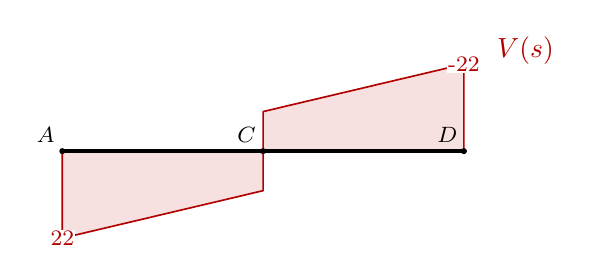
\begin{tikzpicture}[scale=0.850,line join=round]
  \filldraw[fill=red!70!black!12,draw=red!70!black,semithick] (0.000,-1.300) -- (0.125,-1.270) -- (0.250,-1.241) -- (0.375,-1.211) -- (0.500,-1.182) -- (0.625,-1.152) -- (0.750,-1.123) -- (0.875,-1.093) -- (1.000,-1.064) -- (1.125,-1.034) -- (1.250,-1.005) -- (1.375,-0.975) -- (1.500,-0.945) -- (1.625,-0.916) -- (1.750,-0.886) -- (1.875,-0.857) -- (2.000,-0.827) -- (2.125,-0.798) -- (2.250,-0.768) -- (2.375,-0.739) -- (2.500,-0.709) -- (2.625,-0.680) -- (2.750,-0.650) -- (2.875,-0.620) -- (3.000,-0.591) -- (3.000,0.591) -- (3.125,0.620) -- (3.250,0.650) -- (3.375,0.680) -- (3.500,0.709) -- (3.625,0.739) -- (3.750,0.768) -- (3.875,0.798) -- (4.000,0.827) -- (4.125,0.857) -- (4.250,0.886) -- (4.375,0.916) -- (4.500,0.945) -- (4.625,0.975) -- (4.750,1.005) -- (4.875,1.034) -- (5.000,1.064) -- (5.125,1.093) -- (5.250,1.123) -- (5.375,1.152) -- (5.500,1.182) -- (5.625,1.211) -- (5.750,1.241) -- (5.875,1.270) -- (6.000,1.300) -- (6.000,0.000) -- (5.875,0.000) -- (5.750,0.000) -- (5.625,0.000) -- (5.500,0.000) -- (5.375,0.000) -- (5.250,0.000) -- (5.125,0.000) -- (5.000,0.000) -- (4.875,0.000) -- (4.750,0.000) -- (4.625,0.000) -- (4.500,0.000) -- (4.375,0.000) -- (4.250,0.000) -- (4.125,0.000) -- (4.000,0.000) -- (3.875,0.000) -- (3.750,0.000) -- (3.625,0.000) -- (3.500,0.000) -- (3.375,0.000) -- (3.250,0.000) -- (3.125,0.000) -- (3.000,0.000) -- (3.000,0.000) -- (2.875,0.000) -- (2.750,0.000) -- (2.625,0.000) -- (2.500,0.000) -- (2.375,0.000) -- (2.250,0.000) -- (2.125,0.000) -- (2.000,0.000) -- (1.875,0.000) -- (1.750,0.000) -- (1.625,0.000) -- (1.500,0.000) -- (1.375,0.000) -- (1.250,0.000) -- (1.125,0.000) -- (1.000,0.000) -- (0.875,0.000) -- (0.750,0.000) -- (0.625,0.000) -- (0.500,0.000) -- (0.375,0.000) -- (0.250,0.000) -- (0.125,0.000) -- (0.000,0.000) -- cycle;
  \draw[line width=1.6pt] (0.000,0.000) -- (3.000,0.000) -- (6.000,0.000);
  \node[red!70!black,font=\footnotesize,fill=white,inner sep=0.5pt] at (0.000,-1.300) {22};
  \node[red!70!black,font=\footnotesize,fill=white,inner sep=0.5pt] at (6.000,1.300) {-22};
  \fill (0.000,0.000) circle (1.3pt);
  \node[font=\footnotesize] at (0.000,0.000) [xshift=-6pt,yshift=6pt] {$A$};
  \fill (3.000,0.000) circle (1.3pt);
  \node[font=\footnotesize] at (3.000,0.000) [xshift=-6pt,yshift=6pt] {$C$};
  \fill (6.000,0.000) circle (1.3pt);
  \node[font=\footnotesize] at (6.000,0.000) [xshift=-6pt,yshift=6pt] {$D$};
  \node[red!70!black,right] at (6.35,1.50) {$V(s)$};
\end{tikzpicture}\\[5pt]
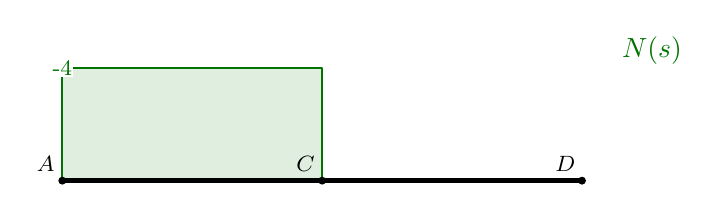
\begin{tikzpicture}[scale=1.100,line join=round]
  \filldraw[fill=green!45!black!12,draw=green!45!black,semithick] (0.000,1.300) -- (0.125,1.300) -- (0.250,1.300) -- (0.375,1.300) -- (0.500,1.300) -- (0.625,1.300) -- (0.750,1.300) -- (0.875,1.300) -- (1.000,1.300) -- (1.125,1.300) -- (1.250,1.300) -- (1.375,1.300) -- (1.500,1.300) -- (1.625,1.300) -- (1.750,1.300) -- (1.875,1.300) -- (2.000,1.300) -- (2.125,1.300) -- (2.250,1.300) -- (2.375,1.300) -- (2.500,1.300) -- (2.625,1.300) -- (2.750,1.300) -- (2.875,1.300) -- (3.000,1.300) -- (3.000,0.000) -- (3.125,0.000) -- (3.250,0.000) -- (3.375,0.000) -- (3.500,0.000) -- (3.625,0.000) -- (3.750,0.000) -- (3.875,0.000) -- (4.000,0.000) -- (4.125,0.000) -- (4.250,0.000) -- (4.375,0.000) -- (4.500,0.000) -- (4.625,0.000) -- (4.750,0.000) -- (4.875,0.000) -- (5.000,0.000) -- (5.125,0.000) -- (5.250,0.000) -- (5.375,0.000) -- (5.500,0.000) -- (5.625,0.000) -- (5.750,0.000) -- (5.875,0.000) -- (6.000,0.000) -- (6.000,0.000) -- (5.875,0.000) -- (5.750,0.000) -- (5.625,0.000) -- (5.500,0.000) -- (5.375,0.000) -- (5.250,0.000) -- (5.125,0.000) -- (5.000,0.000) -- (4.875,0.000) -- (4.750,0.000) -- (4.625,0.000) -- (4.500,0.000) -- (4.375,0.000) -- (4.250,0.000) -- (4.125,0.000) -- (4.000,0.000) -- (3.875,0.000) -- (3.750,0.000) -- (3.625,0.000) -- (3.500,0.000) -- (3.375,0.000) -- (3.250,0.000) -- (3.125,0.000) -- (3.000,0.000) -- (3.000,0.000) -- (2.875,0.000) -- (2.750,0.000) -- (2.625,0.000) -- (2.500,0.000) -- (2.375,0.000) -- (2.250,0.000) -- (2.125,0.000) -- (2.000,0.000) -- (1.875,0.000) -- (1.750,0.000) -- (1.625,0.000) -- (1.500,0.000) -- (1.375,0.000) -- (1.250,0.000) -- (1.125,0.000) -- (1.000,0.000) -- (0.875,0.000) -- (0.750,0.000) -- (0.625,0.000) -- (0.500,0.000) -- (0.375,0.000) -- (0.250,0.000) -- (0.125,0.000) -- (0.000,0.000) -- cycle;
  \draw[line width=1.6pt] (0.000,0.000) -- (3.000,0.000) -- (6.000,0.000);
  \node[green!45!black,font=\footnotesize,fill=white,inner sep=0.5pt] at (0.000,1.300) {-4};
  \fill (0.000,0.000) circle (1.3pt);
  \node[font=\footnotesize] at (0.000,0.000) [xshift=-6pt,yshift=6pt] {$A$};
  \fill (3.000,0.000) circle (1.3pt);
  \node[font=\footnotesize] at (3.000,0.000) [xshift=-6pt,yshift=6pt] {$C$};
  \fill (6.000,0.000) circle (1.3pt);
  \node[font=\footnotesize] at (6.000,0.000) [xshift=-6pt,yshift=6pt] {$D$};
  \node[green!45!black,right] at (6.35,1.50) {$N(s)$};
\end{tikzpicture}\\[10pt]
\end{center}
\end{document}